\documentclass[a4paper,12pt]{article}
\input{framework/Setup}

\def\Titel{\fontsize{20}{30} \selectfont Entwicklung und Evaluierung einer Spiele-KI für „Ganz schön clever“ mittels Deep Reinforcement Learning}
\def\Dozent{Prof. Dr. Mittag, Florian}

% Infos zum Autor
\def\Autorenname{Schubert, Sander}
\def\Geburtsdatum{02.12.1994}
\def\Matrikelnummer{01550217}
\def\Studiengang{Informatik Bachelor}

% Infos zum Unternehmen
\def\Unternehmen{}
\def\Abteilung{}
\def\Strasse{}
\def\Ort{}

% Infos zum Betreuer
\def\Betreuer{Florian Mittag}
\def\Funktion{Betreuer}
\def\Telefon{+49 (0)9561 317-316}
\def\Email{Florian.Mittag@hs-coburg.de}

% Daten
\def\Beginn{<BEGINN>}
\def\Ende{<ENDE>}
\def\Abgabe{\today}


\startHSCdocument[Bachelorarbeit]

CPU: Central Processing Unit

CUDA: Compute Unified Device Architecture

GPU: Graphics Processing Unit

KI: Künstliche Intelligenz

PPO: Proximal Policy Optimization

ReLU: Rectified Linear Unit

TRPO: Trusted Region Policy Optimization
\section{Einleitung}
\subsection{Hinführung zum Thema}
In den vergangenen Jahren gewann Künstliche Intelligenz und insbesondere maschinelles Lernen mit steigender Tendenz an Bedeutung \cite{statista_aiworldwide}. Eines der präsentesten neuen Tools im Jahr 2023 ist ChatGPT 4. Dieses Tool ist ein Chat-Bot, welcher es dem Benutzer ermöglicht mit ihm zu kommunizieren und ihm Fragen oder Aufgaben zu stellen. Solche Tools ermöglichen es Benutzern zunehmend ihre Tätigkeiten zu vereinfachen und prägen somit das Leben der Menschen zunehmend \cite{tagesschaude_chatgpt_nodate}. In dieser Arbeit wurde ChatGPT 4 ebenfalls als unterstützendes Tool verwendet. Vor allem wurde ChatGPT 4 zur Beantwortung fachlicher Fragen und anfänglich zur Generierung von Code für den Prototypen genutzt. Mit zunehmender Komplexität der zu bearbeitenden Aufgabe sinkt die Verlässlichkeit solcher Tools. Daher ist es wichtig, die Anfragen an den Chat-Bot möglichst präzise zu formulieren und den Aufgabenbereich angemessen einzuschränken, um das Tool nicht zu überfordern.

Auch in der Spielentwicklung nehmen Künstliche Intelligenz und maschinelles Lernen schon seit langem eine zentrale Rolle ein \cite{noauthor_kunstliche_2023,millington_ai_2019}. In vielen Spielen gibt es eine oder mehrere Künstliche Intelligenzen, welche bestimmte Aufgaben erfüllen, um den Spieler bei Spiel zu unterstützen oder ihm als Widersacher zu dienen. Auch hier gilt je komplexer die Aufgabenstellung desto schwieriger ist es, einen solchen Bot zu generieren, welcher diese gut und richtig lösen kann.

Das Gemeinschaftsspiel \textit{"Ganz schön clever"} ist ein Würfelspiel, das eine hohe Komplexität aufweist. Diese kommt vor allem durch die hohe Anzahl an möglichen Aktionen (dem sogenannte Aktionsraum) für den Spieler und die vielen Zusammenhänge des Belohnungssystems im Spiel zustande. Das Spiel weist zusätzlich eine hohe Stochastizität auf, welche die Komplexität weiter erhöht.

Interessant ist, wie man für ein solches komplexes Spiel einen Bot oder eine Künstliche Intelligenz entwickeln kann, um dieses gut spielen zu können. Dabei könnte die Komplexität der Aufgabenstellung möglicherweise zu groß sein, um vom Bot erfasst zu werden und es können sich zahlreiche weitere Problemstellungen ergeben, für die Lösungen gefunden werden müssen.
\subsection{Zielsetzung und Motivation}
Ziel der Arbeit ist es, einen Bot beziehungsweise eine Künstliche Intelligenz zu entwickeln, welche das Spiel \textit{"Ganz schön clever"} möglichst gut spielen kann. Gut heißt hierbei, dass im Durchschnitt eine möglichst hohe Punktezahl im Spiel erzielen wird. Es soll analysiert werden, welche Aspekte es bei der Entwicklung zu beachten gilt und wie sich unterschiedliche Ansätze auf das Verhalten und die Performanz der Künstlichen Intelligenz auswirken.

Es gibt noch keine Untersuchungen zu einer Spiel-KI für das Spiel \textit{"Ganz schön clever"}, daher ist es interessant Erkenntnisse darüber zu gewinnen, welche Schwierigkeiten sich hierbei ergeben und wie diese überwunden werden können.
\subsection{Aufgabenstellung}
Es ist eine Künstliche Intelligenz für das Spiel \textit{"Ganz schön clever"} zu implementieren. Hierbei sollen der Vorgang sowie die Ergebnisse des Prozesses analysiert und bewertet werden. Hierzu wird zunächst ein Prototyp entwickelt, welcher eines der fünf Felder des Spiels beinhaltet. Dieser Prototyp soll Einsichten über die Machbarkeit und die Rahmenbedingungen des Projektes bringen. Daraufhin werden die Künstliche Intelligenz und die Spielumgebung schrittweise um ihre jeweiligen Funktionalitäten erweitert, bis das Spiel vollständig und möglichst gut von der Künstlichen Intelligenz gespielt werden kann.
\subsection{Aufbau der Arbeit}
Kapitel 2 beinhaltet einen Grundlagenteil, in dem zunächst das Spiel \textit{"Ganz schön clever"} und seine Mechaniken erklärt werden. Anschließend werden maschinelles Lernen, Reinforcement Learning, Deep Learning und Proximal Policy Optimization behandelt, um eine fachliche Grundlage für das Verständnis der Abläufe beim Training der Künstlichen Intelligenz zu bieten. Im Folgenden werden die verwendeten Technologien des Projektes behandelt. Die vorgestellten Technologien sind Gynmansium, Stable Baselines 3, Matplotlib und ChatGPT 4.

Kapitel 3 befasst sich mit den Anforderungen und der Konzeption des Projektes. Es werden Rahmenbedingungen des Projektes sowie die Anforderungen und die Konzeption für die Spielumgebung und die Künstliche Intelligenz behandelt.

Kapitel 4 zeigt und erklärt die Implementierung des Projektes. Dabei werden die Variablen und Methoden des Projektes erläutert und beschrieben. Zu einem großen Teil wird Pseudocode verwendet, um die Implementierung verständlicher zu machen und den Umfang zu begrenzen.

Kapitel 5 befasst sich mit den Ergebnissen des Projektes, wobei zunächst der Verlauf der Implementierung und dessen einzelne Meilensteine behandelt werden. Ein Prototyp wurde erstellt und anschließend schrittweise erweitert. Daraufhin folgen die Analyse und Darstellung des finalen Modells.

Das abschließende Kapitel 6 beinhaltet eine Zusammenfassung der Arbeit und Anreize zur Weiterarbeit am Projekt.
\section{Grundlagen}
\subsection{Allgemeine Grundlagen}
\subsubsection{Ganz schön clever}
\subsubsection{Machine Learning}
\subsubsection{Reinforcement Learning}
\subsubsection{Deep Learning}
\subsubsection{Proximal Policy Optimization}
\subsection{Verwendete Technologien}
\subsubsection{Gymnasium}
\subsubsection{Stable Baselines 3}
\subsubsection{Matplotlib}
\subsubsection{ChatGPT 4}
\section{Anforderungen und Konzeption}
\subsection{Anforderungen}
Dieses Kapitel beschreibt die Anforderungen des Projektes. Das Projekt ist die Implementierung und die Analyse einer Spiel-KI für das Spiel \textit{"Ganz schön clever"}.
\subsubsection{Rahmenbedingungen}
Es ist eine Künstliche Intelligenz zu implementieren, welche das Spiel \textit{"Ganz schön clever"} gut spielen können soll. Dazu muss zunächst die Spielumgebung entwickelt und implementiert werden. Mithilfe dieser soll ein Verfahren entwickelt werden, welches die Künstliche Intelligenz in dieser Umgebung trainieren soll.

Anschließend sind die Ergebnisse des Entwicklungsprozesses sowie des Erzeugnisses selbst zu analysieren und vorzustellen. Dies soll mithilfe geeigneter, schlüssiger sowie verständlicher Methoden und Visualisierungstechniken erfolgen.
\subsubsection{Spiel}
Das Spiel heißt \textit{"Ganz schön clever"}. Ziel des Spiels ist es, möglichst viele Punkte innerhalb einer vorgeschriebenen Rundenanzahl zu erreichen [siehe Unterabschnitt 2.1.1].

Zunächst soll ein Prototyp der Spielumgebung entwickelt werden, welcher später schrittweise erweitert werden soll, bis das Spiel mit allen Funktionalitäten implementiert worden ist.\\

Diese Funktionalitäten sind:
\begin{itemize}
\item Die sechs farbigen Würfel, welche geworfen werden können und zufällig eine Würfelzahl von 1 bis 6 liefern. Es werden dabei immer alle aktuell gültigen Würfel gleichzeitig geworfen.

\item Ein Mechanismus, welcher die Würfel für die aktuelle Runde als ungültig markiert, sobald sie gewählt werden. Ungültige Würfel dürfen nicht gewählt werden [siehe Unterabschnitt 2.1.1].

\item Ein Mechanismus, welcher Würfel mit einer niedrigeren Augenzahl als der aktuell gewählte Würfel als ungültig für die Runde markiert, solange sich das Spiel nicht in einer Wahl vom Silbertablett oder einer Wahl mithilfe des Extra-Wahl-Bonus befindet.

\item Ein Runden-System, bei dem insgesamt sechs Runden gespielt werden, in denen jeweils bis zu drei Würfe erfolgen, solange bei einem der Würfe noch gültige Würfel vorhanden sind. Zudem erfolgt nach jeder Runde die Auswahl eines Würfels vom Silbertablett, welches die ungültigen Würfel eines anderen Spielers beinhaltet. Wenn das Spiel alleine gespielt wird und es dadurch keinen anderen Spieler gibt, werden hierzu alle Würfel geworfen und drei davon auf das Silbertablett gelegt. Außerdem werden Boni am Anfang der ersten, zweiten, dritten und vierten Runde für alle Spieler freigeschaltet [siehe Unterabschnitt 2.1.1].

\item Die fünf farbigen Felder, gelb, blau, grün, orange und lila. Jedes Feld hat seine eigenen Regeln, wenn es darum geht wann ein Würfel gewählt werden darf, um eines der Kästchen auf diesem Feld auszufüllen [siehe Unterabschnitt 2.1.1]. Die Felder beinhalten verschiedene Belohnungen, die freigespielt werden, wenn bestimmte Kästchen oder Kombinationen aus diesen ausgefüllt worden sind [siehe Unterabschnitt 2.1.1].

\item Die zehn verschiedenen Boni, Fuchs, Extra-Wahl, Neu-Würfeln, Gelbes-Kreuz, Blaues-Kreuz, Grünes-Kreuz, Orangene-Vier, Orangene-Fünf, Orangene-Sechs sowie Lila-Sechs [siehe Unterabschnitt 2.1.1]. Dies beinhaltet sowohl das Erhalten, Speichern, sowie die Benutzung der Boni.

\item Ein Mechanismus, welcher Würfel, die mithilfe eines Extra-Wahl-Bonus gewählt wurden, als ungültig markiert, damit diese nicht erneut in der selben Runde durch mit einem Extra-Wahl-Bonus gewählt werden können.

\item Ein Mechanismus, der Würfel zur richtigen Zeit wieder als gültig markiert. Dies erfolgt nach dem dritten Wurf in der Runde, nach Extra-Wahlen im eigenen Zug (nach dem dritten Wurf), nach der Wahl vom Silbertablett des Gegners und nach Extra-Wahlen, die nach der Wahl vom Silbertablett des Gegners erfolgen. Würfel werden nicht nach jedem Einsatz eines Extra-Wahl-Bonus wieder gültig, sondern erst nachdem der Spieler keinen weiteren Extra-Wahl-Bonus mehr hat oder sich entscheidet zum gegebenen Zeitpunkt keinen weiteren zu verwenden.
\end{itemize}
\subsubsection{Künstliche Intelligenz}
Die Künstliche Intelligenz soll das Spiel möglichst gut spielen können. Es sollen geeignete Methoden zur Verfügung stehen, um die KI trainieren und mit ihr nach dem Training Vorhersagen [siehe Unterabschnitt 2.1.2] treffen zu können. Außerdem sollte sie Möglichkeiten bieten verschiedene Parameter anzupassen, um den Trainingsprozess zu optimieren.

Die wichtigsten dieser Parameter sind unter Anderem:
\begin{itemize} 
\item Trainingsdauer, welche festlegt, wie lange trainiert wird.
\item Gamma, welches bestimmt, wie zukunftsorientiert die KI ihre Entscheidungen fällt. 
\item Die Größe und Art des neuronalen Netzes, das verwendet wird, welches bestimmt, wie genau und präzise Merkmale von der Künstlichen Intelligenz erfasst werden können.
\item Mindestens einen Faktor, welcher das Ausmaß von Erkundung und Ausbeutung steuern soll. 
\end{itemize}
Außerdem soll die Implementierung auf einfache Art und Weise möglich sein, damit der zeitliche Rahmen der Arbeit eingehalten werden kann.
\subsection{Konzeption}
In diesem Kapitel wird das Grundkonzept der Künstlichen Intelligenz sowie der Spielumgebung und deren Zusammenspiel beschrieben.\\

Abbildung 6 zeigt das Zusammenspiel von Spielumgebung und KI während des Trainingsprozesses:

\nopagebreak
\begin{figure}[H]
	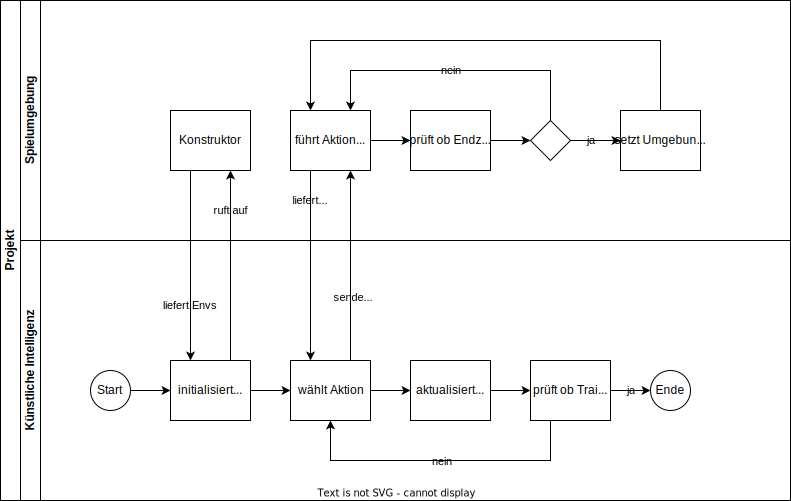
\includegraphics[width=1\textwidth]{Bilder/swimlane.drawio.pdf} 
	\caption[Swimlane-Diagramm des Trainingsprozesses der KI]{Swimlane-Diagramm des Trainingsprozesses der KI\\ Quelle: Eigene Darstellung}
\end{figure}	

Wie Abbildung 6 zeigt wird zunächst der Trainingsprozess angestoßen und die Umgebung wird initialisiert. Dazu wird der Konstruktor der Umgebung aufgerufen. Daraufhin wird eine Aktion von der KI ausgewählt und an die Umgebung weitergeleitet. Die Umgebung führt diese Aktion aus und prüft ob der Endzustand des Spiels erreicht wurde oder nicht. Wenn der Endzustand erreicht wurde, wird die Umgebung auf ihren Anfangszustand zurückgesetzt. Wenn der Endzustand nicht erreicht worden ist, wird der Prozess ohne Weiteres fortgesetzt. Daraufhin liefert die Umgebung der KI eine Belohnung [siehe Unterabschnitt 2.1.3] für den ausgeführten Schritt und den neuen Zustand der Umgebung nach Ausführung der Aktion.

Daraufhin aktualisiert die Künstliche Intelligenz ihr neuronales Netz mit der Policy und überprüft ob bereits genügend Zeit vergangen ist, um das Training zu beenden. Wenn die festgelegte Zeit vergangen ist wird das Training an dieser Stelle beendet. Wenn nicht wird die nächste Aktion gewählt und das Training wird fortgesetzt.

Dies ist lediglich eine vereinfachte Darstellung des Prozesses. In Wirklichkeit wird die Policy nicht nach jedem Schritt/jeder Aktion aktualisiert, sondern es wird erst eine festgelegte Menge an Aktions-Zustands-Paaren gesammelt. Dann wird das neuronale Netz mit dieser Gesamtmenge aktualisiert. Diese Aktions-Zustands-Paare ermöglichen es festzustellen, welche Aktionen in welchen Zuständen zu einem guten Ergebnis führten und welche nicht. Hierfür wird für jeden Zustand ein geschätzter Wert über seinen zukünftigen Nutzen erstellt. Dafür wird ein neuronales Netz, das sogenannte Value Network genutzt. Dieser geschätzte Nutzen wird mit dem tatsächlich erzielten Nutzen verglichen. Die Policy wird anschließend in Richtung vorteilhafter Zustände angepasst, die einen möglichst besseren tatsächlichen als erwarteten Nutzen aufweisen.
\subsubsection{Spielumgebung}
Die Abbildungen 7 und 8 zeigen den prinzipiellen Funktionsablauf in der Spielumgebung. Dabei wird am Anfang eine Aktion entgegengenommen und am Schluss der neue Zustand dieser Umgebung nach Ausführung der Aktion zurückgegeben:
\nopagebreak
\begin{figure}[H]
	\centering
	\includegraphics[width=0.9\textwidth]{Bilder/step3.drawio} 
	\caption[Ablauf-Diagramm der Schritt-Funktion 1]{Ablauf-Diagramm der Schritt Funktion 1\\ Quelle: Eigene Darstellung}
\end{figure}	

Wie Abbildung 7 zeigt wird der Vorgang durch eine Aktion angestoßen. Nach dem Anstoßen, werden die Variablen der Funktion zurückgesetzt, um einen klaren Schnitt zwischen vergangenen Aktionen und der aktuellen Aktion zu erzielen.

Anschließend wird die Aktion ihrem entsprechenden Ablauf zugeordnet. Es gibt Aktionen für Wahlen nach normalen Würfen, für Wahlen von Würfeln des Silbertablettes sowie für das Nutzen von Boni. Außerdem gibt es eine Aktion, die nur dann wählbar ist, wenn keine der anderen Aktionen gewählt werden kann. Dies ist die Aktion für ungültige Züge.

Ist die Aktion nicht gültig, wird die Runde inkrementiert und der Zustand der Umgebung zurückgegeben.

Wird die Neu Würfeln Boni verwendet, werden die gültigen Würfel neu geworfen und anschließend der Zustand zurückgegeben.

Ist beides nicht der Fall kommt es zu einer Auswahl zwischen den wesentlichen Aktionen der Umgebung. Es gibt sogenannte Extra-Wahlen. Diese spalten sich auf in Extra-Wahlen mit einem Extra-Wahl-Bonus und Wahlen vom Silbertablett eines Mitspielers.

Handelt es sich nicht um eine Extra-Wahl, so folgt eine Unterteilung in Extra-Runden und Normale-Runden. Bei Extra-Runden wird eine der Boni verwendet (in Abb. 8: Boni Wahl), die es erlauben eines der farbigen Felder direkt auszufüllen [siehe Unterabschnitt 2.1.1].

Handelt es sich nicht um eine Extra-Runde muss es sich in diesem Fall um eine Normale-Runde (in Abb. 8: Normale Wurf Wahl) nach einem gewöhnlichen Wurf handeln [siehe Abb. 2].

Handelt es sich um eine Extra-Wahl mit Boni (mit Extra-Wahl-Bonus), dann steht noch die Aktion "Passen" zur Wahl. Diese inkrementiert lediglich die Runde, sodass das Spiel weiter fortgesetzt werden kann. Dies spiegelt die Möglichkeit im Spiel wieder auf die Nutzung eines Extra-Wahl-Bonus zu verzichten.\\

\begin{figure}[H]
	\centering
	\includegraphics[width=0.9\textwidth]{Bilder/step2.drawio} 
	\caption[Ablauf-Diagramm der Schritt-Funktion 2]{Ablauf-Diagramm der Schritt Funktion 2\\ Quelle: Eigene Darstellung}
\end{figure}

Wie in Abbildung 8 dargestellt gestaltet sich der folgende Ablauf der Funktion relativ ähnlich bei allen vier Varianten. Es wird das Feld und das Kästchen ermittel, welches ausgefüllt werden soll und das entsprechende Kästchen wird anschließend ausgefüllt. Dann wird die Belohnung für diesen Schritt ermittelt.

Am Ende der Funktion unterscheiden sich die vier Varianten wieder. Bei einer Normalen-Runde nach einem normalen Wurf werden die entsprechenden Würfel als ungültig markiert [siehe Unterabschnitt 2.1.1] und die Runde wird inkrementiert. Außerdem prüft die Funktion bei dieser Variante am Ende, ob das Spiel terminiert ist oder nicht.

Beim Ausfüllen eines Feldes mittels eines Bonus (kein Extra-Wahl-Bonus) wird der entsprechende Bonus dekrementiert.

Bei der Extra-Wahl vom Silbertablett wird die Runde inkrementiert.

Bei der Extra-Wahl mittels Bonus wird der gewählte Würfel als ungültig markiert und der Extra-Wahl-Bonus dekrementiert.

Bei allen vier Varianten wird am Ende der Funktion der aktuelle Zustand der Umgebung sowie die erhaltene Belohnung für den Schritt zurückgegeben.

\subsubsection{Künstliche Intelligenz}
Abbildung 9 zeigt die wesentlichen Hyperparameter, die bei der Entwicklung der Künstlichen Intelligenz von Bedeutung sind:
\nopagebreak
\begin{figure}[H]
	\centering
	\includegraphics[width=0.6\textwidth]{Bilder/KI} 
	\caption[Wesentliche Hyperparameter der Künstlichen Intelligenz]{Wesentliche Hyperparameter der Künstlichen Intelligenz\\ Quelle: Eigene Darstellung}
\end{figure}

Die Künstliche Intelligenz basiert auf der MaskablePPO-Version von Stable Baselines 3 Contributing. Es sind Konfigurationen zu treffen, welche das Training beeinflussen und steuern. Diese Einstellungen werden Hyperparameter genannt. Hyperparameter legen die Ausprägung gewisser Steuerelemente des MaskablePPO-Algorithmus und ähnlicher Reinforcement-Learning-Algorithmen fest.

Die wichtigsten Hyperparameter für das Projekt sind folgende [siehe Abb. 9]:

\begin{itemize} 
\item Netzwerkarchitektur: Legt die Anzahl der Schichten des neuronale Netzes fest, Dieses Netz wird zur Abbildung der Policy verwendet. Außerdem legt die Netzwerkarchitektur fest, wie viele Neuronen es pro Schicht gibt [siehe Unterabschnitt 2.1.4]. Die Netzwerkarchitektur ist so zu bestimmen, dass die Künstliche Intelligenz im Stande ist, die Komplexität der Problemstellung zu erfassen und gleichzeitig zu gewährleisten, dass die Trainingsdauer und die Systemauslastung dadurch nicht zu hoch steigen. Außerdem sollte es nicht zu einer Überanpassung an die Trainingsdaten kommen. Da es sich bei dem neuronalen Netz um ein Multilayer Perceptron handelt, sind alle Neuronen einer Schicht mit allen der vorherigen und folgenden Schicht verbunden [siehe Unterabschnitt 2.1.4]. Dies führt dazu, dass die Rechenleistung für das Updaten der Gewichte der Policy exponentiell steigt, je komplexer das neuronale Netz wird. Dies führt zu einer gesteigerten Trainingsdauer und Systemauslastung. Außerdem tendieren zu komplexe Neuronale Netze dazu, sich stark an die Trainingsdaten anzupassen, was zu Überanpassung führen kann. Zu komplexe Netze generalisieren tendenziell schlechter auf neue Datensätze, die sich stark von den Trainingsdaten unterscheiden.

\item Anzahl der Umgebungen: Eine erhöhte Anzahl an Trainingsumgebungen ermöglicht es, besonders bei Nutzung von CUDA (GPU), parallel Daten aus mehreren Umgebungen zu sammeln und zu verarbeiten. Dies erhöht die Trainingsgeschwindigkeit, da ein erheblicher Teil der Trainingsdauer in diesem Projekt davon abhängt, wie schnell die nötigen Trainingsdaten aus den Umgebungen generiert werden können. Außerdem erhöht die Nutzung von CUDA die Geschwindigkeit von Policy Updates enorm, da viele der Berechnungen im neuronalen Netz parallel abgearbeitet werden können. Allerdings erhöht die Anzahl der Umgebungen die RAM Auslastung enorm und die CPU Auslastung mittelmäßig stark, was dazu führt, dass es ineffizient wäre auf dem verwendeten System (Nvidia Geforce GTX 1070, Intel i5 8600k, 16GB RAM) deutlich mehr als 32 Umgebungen zu betreiben.

\item Aktivierungsfunktion: Legt zusammen mit den Gewichtungen der Neuronen fest, wann und wie stark diese ihre Signale an die folgenden Neuronen weiterleiten. Im Projekt wird vor allem die ReLU-Funktion verwendet, da diese standardmäßig vom Algorithmus verwendet wird und im allgemeinen sowie spezifisch in diesem Projekt gute Ergebnisse erzielt. Die Formel der ReLU-Funktion lautet: f(x) = max(0,x). Die ReLU-Funktion gibt, wenn der Wert kleiner als Null ist, Null zurück und ansonsten den Wert selbst \cite{schmidt-hieber_nonparametric_2020}.
\end{itemize} 

Abbildung 10 zeigt den Graphen der ReLU-Funktion:
\nopagebreak
\begin{figure}[H]
	\centering
	\includegraphics[width=0.7\textwidth]{Bilder/ReLU} 
	\caption[Graph der ReLU-Funktion]{Graph der ReLU-Funktion\\ Quelle: Eigene Darstellung}
\end{figure}

\begin{itemize} 
\item Gamma: Legt fest, wie stark zukünftige Belohnungen wertgeschätzt werden. Es fungiert als eine Art Multiplikator. Potenzielle Belohnungen werden pro Spielschritt, den sie in der Zukunft entfernt liegen würden, mit Gamma multipliziert. Gamma ist so zu wählen, dass das Modell lernt, die bestmöglichen Aktionen zu wählen, um insgesamt das beste Ergebnis zu erzielen. Zu hohe Werte von Gamma können dazu führen, dass kurzzeitige Belohnungen vernachlässigt werden, was zu einem schlechteren Gesamtergebnis führen kann, wenn diese von besonderer Bedeutung sind. Zu niedrige Werte von Gamma können wiederum dazu führen, dass der Agent nicht zukunftsorientiert handelt und somit kein gutes Gesamtergebnis erzielt, da er sich hauptsächlich auf kurzfristige Belohnungen konzentriert, anstatt in die Zukunft zu schauen und dieser Wert zuzumessen. In diesem Projekt bewegt sich der Wert von Gamma im Allgemeinen in einem Bereich zwischen 0.5 und 1.

\item Lernrate: Bestimmt, wie stark Updates des neuronalen Netzes und seiner Gewichtungen pro Updateschritt ausfallen. Zu große Werte für die Lernrate können zu einem instabilen Training führen, da die Updates somit stark vom Trainingsdatensatz abhängen. Zu niedrige Werte führen wiederum zu einer Erhöhung der benötigten Trainingsdaten und Trainingsdauer. Der Wert für die Lernrate bewegt sich im Projekt üblicherweise zwischen Werten von 0.0003 bis zu 0.0003x32.

\item Entropie-Koeffizient: Bestimmt das Maß an Exploration des Modells. Je höher der Entropie-Koeffizient ist desto stärker Belohnt das Modell neue beziehungsweise bisher wenig erkundete Aktionen oder Zustände. Ein zu hoher Wert führt dazu, dass das Modell nicht lernt bereits funktionierende Taktiken ausreichend zu verfestigen. Ein zu niedriger Wert führt dazu, dass das Modell sich relativ schnell auf eine bisher vergleichsweise gut funktionierende Strategie festlegt und diese verfestigt. Der Entropie-Koeffizient bewegt sich innerhalb des Projektes meist zwischen Werten von 0.05 und 0.3, wobei sich ein Wert um die 0.1 als stabil und effizient herausgestellt hat.

\item Clip-Range: Die Clip-Range ist spezifisch für den PPO-Algorithmus [siehe Unterabschnitt 2.1.5]. Sie legt fest wie stark Policy Updates sein dürfen und ab welchem Schwellwert die Updates abgeschnitten werden. Abschneiden heißt, dass die Updates zwar durchgeführt werden, allerdings darf die Policy nach dem Update nur maximal um einen bestimmten Wert von der vorherigen abweichen. Die standardmäßige Clip-Range beläuft sich auf 0.2. Innerhalb des Projektes werden auch andere Werte getestet.

\item nSteps: Legt fest, wie viele Aktions-Zustands-Paare gesammelt werden, bevor ein Update des neuronales Netzes erfolgt.

\item nEpochs: Legt fest wie oft dasselbe Datenpaket von nSteps für das Training benutzt wird bevor es verworfen wird. Je öfter man es verwendet, desto weniger Daten braucht man und desto schneller verläuft das Training. Allerdings sollte der selbe Datensatz nicht zu häufig verwendet werden, um Überanpassung zu vermeiden. nEpochs hat im Rahmen des Projektes üblicherweise einen Wert zwischen 5 und 11.

\item Batch Size: Das Datenpaket von nSteps wird vor der Verwendung für das Updaten des neuronalen Netzes in kleinere Datenpakete, die sogenannten Batches, zerlegt. Daraufhin werden Updates mit jedem dieser Batches durchgeführt. Die Aufteilung erfolgt per Zufall, daher ist mit hoher Wahrscheinlichkeit keines der Datenpakete (Batches) wie das andere, selbst wenn dasselbe Gesamtdatenpaket durch ein hohes nEpochs viele male verwendet wird. Batch Size legt fest wie groß diese kleineren Datenpakete (Batches) sind.

\item 
Trainingsdauer: Die Trainingsdauer legt fest wie lange trainiert wird. Die Implementierung von Stable Baselines [siehe Kapitel 2.2.2] verwendet standardmäßig Timesteps zur Messung von Zeit. Eine Timestep ist ein ausgeführter Schritt beziehungsweise eine ausgeführte Aktion in einer Umgebung. Die Timesteps von mehreren parallel laufenden Umgebungen werden aufsummiert, somit kommt es nicht zu vermehrtem Training alleine durch Erhöhung der Umgebungsanzahl bei gleichbleibender Trainingsdauer in Timesteps.
\end{itemize}
\section{Implementierung}
In diesem Kapitel wird die Implementierung des Projektes vorgestellt und erläutert. Zur Darstellung der Funktionsweise der einzelnen Funktionen wird Pseudocode verwendet. Dies soll dabei helfen die Funktionsweise verständlicher und knapper aufzuzeigen.
\subsection{Einschränkungen}
Aus zeitlichen Gründen ergeben sich einige Einschränkungen für das Design der Implementierung. Das Spiel endet nach der Wahl des Würfels nach dem dritten Wurf in der sechsten Runde. Somit kann der Extra-Wahl-Bonus kein letztes Mal benutzt werden und es gibt in der letzten Runde auch keine Wahl vom Silbertablett. Außerdem werden nicht die niedrigsten sechs Würfel des Wurfes auf das Silbertablett des Mitspielers gelegt, sondern drei zufällige.
\subsection{Spielumgebung}
Die Implementierung besteht aus zwei Klassen. Eine davon ist die Spielumgebung. Zunächst werden in diesem Kapitel die wesentlichen Attribute der Spielumgebung und anschließend ihre Methoden erläutert. Für die Implementierung der Spielumgebung wurde die Bibliothek Gymnasium [siehe Unterabschnitt 2.2.1] verwendet.
\subsubsection{Klassenattribute}
\begin{minipage}{\linewidth}
Code 1 zeigt die Klassenattribute, die für das Rundenmanagement wichtig sind:
\vspace{0.5cm}
\begin{lstlisting}[caption={Klassenattribute für das Runden-System}, basicstyle=\ttfamily]
self.initial_rounds
self.rounds
self.roll_in_round
\end{lstlisting}
\end{minipage}

Das Attribut \texttt{initial\_rounds} beschreibt die maximale Rundenanzahl des Spiels und wird beim Zurücksetzen der Umgebung verwendet, um die Rundenzahl auf den gewünschten Wert (im Solo-Spiel sechs) zurückzusetzen.

Das Attribut \texttt{rounds} repräsentiert die aktuell verbleibende Rundenanzahl im Spiel.

Das Attribut \texttt{roll\_in\_round} repräsentiert die Nummer des aktuellen Wurfes in der Runde.\\

\begin{minipage}{\linewidth}
Code 2 zeigt die Klassenattribute, die für das Würfeln der Würfel relevant sind:
\vspace{0.5cm}
\begin{lstlisting}[caption={Klassenattribute für Würfel}, basicstyle=\ttfamily]
self.invalid_dice = {"white": False, "yellow": False, ...}
self.dice = {"white": 0, "yellow": 0, ...}
\end{lstlisting}
\end{minipage}

Die Attribute \texttt{invalid\_dice} und dice repräsentieren die Augenzahlen der Würfel, sowie die Gültigkeit der Würfel selbst. Ist der Wert von \texttt{invalid\_dice} False, ist der Würfel nicht ungültig und somit gültig.\\

\begin{minipage}{\linewidth}
Code 3 zeigt die Klassenattribute, die für das bilden einer Punktestandhistorie relevant sind:
\vspace{0.5cm}
\begin{lstlisting}[caption={Klassenattribute für die Nachvollziehbarkeit von Punkteständen}, basicstyle=\ttfamily]
self.score
self.score_history
self.initialized
\end{lstlisting}
\end{minipage}

Das Attribut \texttt{score} repräsentiert den aktuellen Punktestand der Spielumgebung. Es wird verwendet, um erreichte Punktestände in die \texttt{score\_history} einzutragen. Das Attribut \texttt{score\_history} ist eine Historie über die erreichten Punktestände in den einzelnen Episoden beziehungsweise Spieldurchläufen. Das Attribut \texttt{initialized} wird verwendet, um zu gewährleisten, dass nur Einträge in der Punktestandhistorie eingetragen werden, nachdem ein Spiel abgeschlossen wurde. Es trifft eine Aussage darüber ob die Spielumgebung bereits einmal initialisiert wurde oder nicht.\\

\begin{minipage}{\linewidth}
Code 4 zeigt die Klassenattribute, welche die farbigen Felder des Spielbrettes repräsentieren:
\vspace{0.5cm}
\begin{lstlisting}[caption={Klassenattribute für die farbigen Felder des Spiels}, basicstyle=\ttfamily]
self.yellow_field = [[3, 6, 5, 0], [2, 1, 0, 5], ...]
self.blue_field = [[0, 2, 3, 4], [5, 6, 7, 8], [9, 10, 11, 12]]
self.green_field = [0] * 11
self.orange_field = [0] * 11
self.purple_field = [0] * 11
\end{lstlisting}
\end{minipage}

Die Attribute \texttt{yellow\_field}, \texttt{blue\_field}, \texttt{green\_field}, \texttt{orange\_field} und \texttt{purple\_field} stehen für die fünf farbigen Felder auf dem Spielbrett. Sie repräsentieren die eingetragenen Werte auf dem Spielbrett und bestimmen somit welche Kästchen aktuell ausgefüllt werden können (vorausgesetzt die Würfelergebnisse passen) und welche Belohnungen freigeschaltet werden.\\

\begin{minipage}{\linewidth}
Code 5 zeigt die Klassenattribute, welche die zu erspielenden Boni auf den farbigen Feldern repräsentieren:
\vspace{0.5cm}
\begin{lstlisting}[caption={Klassenattribute für freizuschaltende Boni}, basicstyle=\ttfamily]
self.yellow_rewards = {"row": ["blue_cross", ...], "dia": ...}
self.blue_rewards = {"row": ["orange_five", ...], "col": ...}
self.green_rewards = [None, None, None, "extra_pick", ...]
self.orange_rewards = [None, None, "re_roll", ...]
self.purple_rewards = [None, None, "re_roll", ...]
\end{lstlisting}
\end{minipage}

Die Attribute \texttt{yellow\_rewards}, \texttt{blue\_rewards}, \texttt{green\_rewards}, \texttt{orange\_rewards} und \texttt{purple\_rewards} repräsentieren die freizuschaltenden Boni für die jeweiligen farbigen Felder. Für das blaue Feld sind diese in Form von Reihen (\texttt{row}) und Spalten (\texttt{col}) aufgeführt. Das gelbe Feld besitzt Boni für das Ausfüllen von Reihen (\texttt{row}) und einen Boni, der bei diagonalem Ausfüllen (\texttt{dia}) freigeschaltet werden kann. Für die Farben grün, orange und lila sind die Boni jeweils direkt einem der Kästchen im Feld zugewiesen, wobei viele der Kästchen keinen freizuschaltenden Bonus aufweisen, was dem Wert None entspricht.\\

\begin{minipage}{\linewidth}
Code 6 zeigt die Klassenattribute, für die Punktebelohnungen des gelben, blauen und grünen Feldes:
\vspace{0.5cm}
\begin{lstlisting}[caption={Klassenattribute für freizuschaltende Punktebelohnungen des gelben, blauen und grünen Feldes}, basicstyle=\ttfamily]
self.yellow_rewards = {"col": [10, 14, 16, 20], ...}
self.blue_count_rewards = [0, 1, 1, 2, 3, 4, 5, 6, 7, 8, 9, 10]
self.green_count_rewards = [1, 2, 3, 4, 5, 6, 7, 8, 9, 10, 11]
\end{lstlisting}
\end{minipage}

Im Attribut \texttt{yellow\_rewards} sind die Punktebelohnungen im Spaltenbereich (\texttt{col}) des gelben Feldes aufgeführt. Die Attribute \texttt{blue\_count\_rewards} und \texttt{green\_count\_rewards} repräsentieren die Punktebelohnungen, welche erspielt werden können, sobald ein blaues beziehungsweise grünes Kästchen ausgefüllt wird. Beginnend vom ersten Wert des Arrays und danach inkrementell aufsteigend, steigt die erhaltene Punktebelohnung bei jedem ausgefüllten Kästchen stetig an.\\

\begin{minipage}{\linewidth}
Code 7 zeigt die Klassenattribute der Flags für die Belohnungen der farbigen Felder. Sind diese gesetzt und sind die entsprechenden Kästchen für die Belohnung ausgefüllt, wurde die Belohnung bereits ausgeschüttet und wird es nicht erneut, bis die Attribute nach dem Spiel zurückgesetzt werden:
\vspace{0.5cm}
\begin{lstlisting}[caption={Klassenattribute für Belohnungsflags}, basicstyle=\ttfamily]
self.yellow_reward_flags = {"row": [False] * 4, "col": ...}
self.blue_reward_flags = {"row": [False] * 3, "col": ...}
self.blue_count_reward_flags = [False] * 12
self.green_reward_flags = [False] * 11
self.orange_reward_flags = [False] * 11
self.purple_reward_flags = [False] * 11
\end{lstlisting}
\end{minipage}

\begin{minipage}{\linewidth}
Code 8 zeigt die Klassenattribute für Punktestände der einzelnen farbigen Felder. Die Punktewerte werden aufaddiert, sobald Punkte im entsprechenden Feld erspielt worden sind und am Ende genutzt, um den Wert der Fuchs-Boni zu bestimmen [siehe Unterabschnitt 2.1.1]:
\vspace{0.5cm}
\begin{lstlisting}[caption={Klassenattribute für erreichte Punktestände der einzelnen farbigen Felder}, basicstyle=\ttfamily]
self.yellow_field_score
self.blue_field_score
self.green_field_score
self.orange_field_score
self.purple_field_score
\end{lstlisting}
\end{minipage}

\begin{minipage}{\linewidth}
Code 9 zeigt die Klassenattribute für freigeschaltete Boni. Wird eine Boni erspielt, wird ihr Wert inkrementiert, wird sie genutzt, wird er dekrementiert:
\vspace{0.5cm}
\begin{lstlisting}[caption={Klassenattribute für freigespielte Boni}, basicstyle=\ttfamily]
self.extra_pick
self.re_roll
self.fox
self.yellow_cross
self.blue_cross
self.green_cross
self.orange_four
self.orange_five
self.orange_six
self.purple_six
\end{lstlisting}
\end{minipage}

\begin{minipage}{\linewidth}
Code 10 zeigt die Klassenattribute für die Anzahl an gewählten Kästchen in den verschiedenen farbigen Feldern. Wenn ein Kästchen in einem der Felder ausgefüllt wird, wird der Wert des entsprechenden Attributes inkrementiert. Diese Attribute dienen nicht dem Spielablauf selbst, sondern der Nachvollziehbarkeit der Strategie des Modells:
\vspace{0.5cm}
\begin{lstlisting}[caption={Klassenattribute für die Anzahl an gewählte Kästchen innerhalb der farbigen Feldern}, basicstyle=\ttfamily]
self.picked_yellow
self.picked_blue
self.picked_green
self.picked_orange
self.picked_purple
\end{lstlisting}
\end{minipage}

\begin{minipage}{\linewidth}
Code 11 zeigt die Klassenattribute für den Aktions- sowie Beobachtungsraum:
\vspace{0.5cm}
\begin{lstlisting}[caption={Klassenattribute des Aktions- und Beobachtungsraumes}, basicstyle=\ttfamily]
self.number_of_actions = 247
low_bound = np.array([0]*16 + [0]*12 + ...)
high_bound = np.array([6]*16 + [6]*12 + ...)
self.action_space = spaces.Discrete(self.number_of_actions)
self.observation_space = spaces.Box(low_bound, high_bound, ...)
self.valid_action_mask_value = np.ones(self.number_of_actions)
\end{lstlisting}
\end{minipage}

Das Attribut \texttt{number\_of\_actions} repräsentiert die Gesamtanzahl an möglichen Aktionen des Modells. Die Attribute \texttt{low\_bound} und \texttt{high\_bound} setzen die obere und untere Grenze von Werten im Beobachtungsraum fest. Beispielsweise steht der erste Eintrag in beiden für Werte des gelben Feldes. Diese können von null \texttt{([0]*16)} bis sechs \texttt{([6]*16)} reichen. Das Attribut \texttt{action\_space} repräsentiert den Aktionsraum des Modells. Es ist ein diskreter Raum mit \texttt{number\_of\_actions} Werten von null bis \texttt{number\_of\_actions} minus eins. Das Attribut \texttt{observation\_space} repräsentiert den Beobachtungsraum. \texttt{Shape} definiert dabei die Größe des Beobachtungsraumes. Das Attribut \texttt{valid\_action\_mask\_value} repräsentiert die Aktionsmaske. Initial handelt es sich dabei um ein Numpy Array aus Einsen. Einsen stehen für gültige Aktionen, Nullen für ungültige. Die Werte verlaufen parallel zu den Werten des Aktionsraumes. Somit repräsentieren alle Werte (beispielsweise \texttt{[0]} oder \texttt{[5]}) sowohl im Aktionsraum als auch bei der Aktionsmaske die selbe Aktion.\\

Die Struktur des Aktionsraumes ist für das Verständnis der Arbeit wichtig, daher wird sie hier erläutert:

Die ersten 122 Werte des Aktionsraumes von 0 bis 121 sind sowohl normalen Wahlen bei eigenen Würfen als auch den verschiedenen Boni, welche es ermöglichen direkt ein Kästchen eines Felder anzukreuzen, zugeordnet. Dabei stehen die ersten 16 Werte für Kästchen des gelben Feldes, die nächsten 12 für Kästchen des blauen Feldes, und die folgenden 33 zu einer Aufteilung von jeweils 11 für Kästchen im grünen, orangenen und lila Feld. Die Werte von 61 bis 121 stehen für die selben Kästchen in der selben Reihenfolge wie die vorherigen 61 Werte, allerdings wird bei diesen der weiße Würfel verwendet statt des jeweils farbigen Würfels für das spezifische Feld.

Die Werte von 122 bis 243 stehen für Wahlen mit der Extra-Wahl-Boni oder für Wahlen vom Silbertablett des Gegners. Die Struktur innerhalb dieser Reichweite ist die selbe wie bei den 122 Werte zuvor. Die ersten 16 Werte stehen für die selben Kästchen im gelben Feld und so weiter.

Der Wert 244 steht für die Neu Würfeln Boni, der Wert 245 für das Passen bei einem möglichen Einsatz von Extra-Wahl-Boni und der Wert 246 für eine ungültige Aktion, die nur möglich ist, wenn keine der anderen Aktionen getätigt werden kann.
\subsubsection{Schritt-Methode}
Code 12 zeigt die Funktionsweise der Schritt-Methode (\texttt{step method}) der Spielumgebung mithilfe von Pseudocode. Diese Methode führt Spielschritte beziehungsweise Aktionen in der Spielumgebung aus:
\vspace{0.5cm}
\begin{lstlisting}[caption={Schritt-Methode}]
step(Aktion):
	Setze Methodenattribute zurück
	
	if not Extra-Wahl:
		if Aktion im gelben Feld:
			Fülle entsprechendes gelbes Kästchen aus
			if Gelbes-Kreuz-Boni >= 1
				Bonusrunde = True
				Gelbes-Kreuz-Boni -= 1
			if not Bonusrunde:
				Setze entsprechende Würfel auf ungültig
		if Aktion im blauen Feld:
			Fülle entsprechendes blaues Kästchen aus
			if Blaues-Kreuz-Boni >= 1:
				Bonusrunde = True
				Blaues-Kreuz-Boni -= 1
			if not Bonusrunde:
				Setze entsprechende Würfel auf ungültig
		if Aktion im grünen Feld:
			Fülle entsprechendes grünes Kästchen aus
			if Grünes-Kreuz-Boni >= 1:
				Bonusrunde = True
				Grünes-Kreuz-Boni -= 1
			if not Bonusrunde:
				Setze entsprechende Würfel auf ungültig
		if Aktion im orangene Feld:
			Fülle entsprechendes orangenes Kästchen aus
			if Orangene-Feld-Boni >= 1:
				Bonusrunde = True
				Orangene-Feld-Boni -= 1
			if not Bonusrunde:
				Setze entsprechende Würfel auf ungültig
		if Aktion im lila Feld:
			Fülle entsprechendes lila Kästchen aus
			if Lila-Sechs-Boni >= 1:
				Bonusrunde = True
				Lila-Sechs-Boni -= 1
			if not Bonusrunde:
				Setze entsprechende Würfel auf ungültig
	
	if Extra-Wahl:
		Bonusrunde = True
		if Extra-Wahl-Bonus benutzt:
			Extra-Wahl-Boni -= 1
		Finde Kästchen zum ausfüllen und fülle es aus
		Setze gewählten Würfel auf ungültig
		if Extra-Wahl-Boni <= 0 or Wahl erfolgte vom Silbertablett:
			Runde wird inkrementiert
			
	if Neu-Würfeln-Bonus wird benutzt:
		Werfe Würfel neu
		Neu-Würfeln-Boni -= 1
		Aktualisiere Aktionsmaske
		return Beobachtungsraum, Punktebelohnung, Spiel terminiert?
		
	if Statt Extra-Wahl-Boni gepasst wird:
		Runde wird inkrementiert
		return Beobachtungsraum, Punktebelohnung, Spiel terminiert?
	if ungültige Aktion gewählt da keine gültigen Aktionen vorhanden:
		Nichts tun
			
	Punktebelohnung += erspielte Belohnung in diesem Schritt
	if not Bonusrunde:
		Runde wird inkrementiert
		if Rundenanzahl == 0:
			terminiert = True
			Punktebelohnung += Fuchsbonipunktebelohnung
	Aktualisiere Aktionsmaske
	return Beobachtungsraum, Punktebelohnung, Spiel terminiert?		
\end{lstlisting}
\subsubsection{Methode zum Zurücksetzen der Spielumgebung}
\begin{minipage}{\linewidth}
Code 13 zeigt die Funktionsweise der Methode zum Zurücksetzen der Spielumgebung (\texttt{reset method}) mithilfe von Pseudocode. Sie setzt Umgebungen, in denen ein Spiel abgeschlossen wurde, auf den Anfangszustand zurück, damit eine weitere Runde gespielt werden kann:
\vspace{0.5cm}
\begin{lstlisting}[caption={Methode zum Zurücksetzen der Umgebung}]
reset():
	Setze alle Attribute für den Spielablauf auf den Startzustand
\end{lstlisting}
\end{minipage}

\subsubsection{Methode zur Visualisierung der Spielumgebung}
\begin{minipage}{\linewidth}
Code 14 zeigt die Funktionsweise der Funktion zur Visualisierung der Spielumgebung (\texttt{render method}) mithilfe von Pseudocode. Die Visualisierung dient einer verbesserten Nachvollziehbarkeit der Ereignisse innerhalb der Spielumgebung:
\vspace{0.5cm}
\begin{lstlisting}[caption={Methode zur Visualisierung der Spielumgebung}]
render():
	Zeige alle relevanten Attribute und Merkmale der Umgebung an
\end{lstlisting}
\end{minipage}

\subsubsection{Würfel-Methode}
\begin{minipage}{\linewidth}
Code 15 zeigt die Funktionsweise der Methode zum Werfen der Würfel (\texttt{roll\_dice method}) mithilfe von Pseudocode. Würfel müssen nach jedem Wurf, bei Anfang jeder Spielrunde und beim Einsetzen des Neu-Würfeln-Bonus neu geworfen werden:
\vspace{0.5cm}
\begin{lstlisting}[caption={Methode zum Werfen der Würfel}]
roll_dice():
	Werfe Würfel neu
\end{lstlisting}
\end{minipage}

\subsubsection{Methode zur Überprüfung der freigespielten Belohnungen}
\begin{minipage}{\linewidth}
Code 16 zeigt die Funktionsweise der Methode zur Überprüfung der freigespielten Belohnungen (\texttt{check\_rewards method}) mithilfe von Pseudocode. Diese Methode überprüft jedes Mal, nachdem ein Kästchen in der Spielumgebung ausgefüllt worden ist, ob und welche Belohnung freigespielt wurde und fügt diese dem Inventar des Spielers hinzu:
\vspace{0.5cm}
\begin{lstlisting}[caption={Methode zur Überprüfung der freigespielten Belohnungen}]
check_rewards():
	Überprüfe ob im gelben Feld Belohnungen freigeschaltet wurden
	Schalte im gelben Feld freigeschaltete Belohnungen frei
	
	Überprüfe ob im blauen Feld Belohnungen freigeschaltet wurden
	Schalte im blauen Feld freigeschaltete Belohnungen frei
	
	Überprüfe ob im grünen Feld Belohnungen freigeschaltet wurden
	Schalte im grünen Feld freigeschaltete Belohnungen frei
	
	Überprüfe ob im orangenen Feld Belohnungen freigeschaltet wurden
	Schalte im orangenen Feld freigeschaltete Belohnungen frei
	
	Überprüfe ob im lila Feld Belohnungen freigeschaltet wurden
	Schalte im lila Feld freigeschaltete Belohnungen frei
	
	return Punktebelohnung
\end{lstlisting}
\end{minipage}

\subsubsection{Methode zur Generierung des Beobachtungsraumes}
\begin{minipage}{\linewidth}
Code 17 zeigt die Funktionsweise der Methode zur Generierung des Beobachtungsraumes (\texttt{\_get\_obs method}) mithilfe von Pseudocode. Diese Methode vereinfacht es, den Beobachtungsraum zu generieren, welcher jedes Mal benötigt wird, wenn ein Schritt in der Umgebung ausgeführt wird:
\vspace{0.5cm}
\begin{lstlisting}[caption={Methode zur Generierung des Beobachtungsraumes}]
_get_obs():
	Erstelle Numpy Arrays für farbige Felder
	Erstelle Numpy Array für Würfelergebnisse
	Erstelle Numpy Array für ungültige Würfel
	Füge Arraywerte für Boni und Rundenzahl hinzu
	Beobachtungsraum = Verbinde alle Arrays miteinander
	
	return Beobachtungsraum
\end{lstlisting}
\end{minipage}

\subsubsection{Methode zur Generierung der Aktionsmaske}
Code 18 zeigt Die Funktionsweise der Methode zur Generierung der Aktionsmaske (\texttt{valid\_action\_mask method}) mithilfe von Pseudocode. Einsen stehen für gültige Aktionen und Nullen für ungültige. Die Wahlwahrscheinlichkeit des Modells für ungültige Aktionen wird auf null gesetzt:
\vspace{0.5cm}
\begin{lstlisting}[caption={Methode zur Generierung der Aktionsmaske}]
valid_action_mask():
	Setze alle Werte auf Eins
	
	Werte für bereits ausgefüllte gelbe Kästchen = 0
	Werte für gelbe Kästchen ohne passende Würfelergebnisse = 0
	
	Werte für bereits ausgefüllte blaue Kästchen = 0
	Werte für blaue Kästchen ohne passende Würfelergebnisse = 0
	
	Werte für bereits ausgefüllte grüne Kästchen = 0
	Werte für grüne Kästchen ohne passende Würfelergebnisse = 0
	
	Werte für bereits ausgefüllte orangene Kästchen = 0
	Werte für orangene Kästchen ohne passende Würfelergebnisse = 0
	
	Werte für bereits ausgefüllte lila Kästchen = 0
	Werte für lila Kästchen ohne passende Würfelergebnisse = 0
	
	Werte für Akionen mithilfe ungültiger Würfel = 0
	
	if not Extra-Wahl or ungültige Extra-Wahl:
		Werte von 122 bis 243 & Wert für das Aussetzen = 0
	if gültige Extra-Wahl:
		Werte von 0 bis 121 = 0
		Wert für das Aussetzen = 1
	
	if Neu-Würfeln-Boni <= 0 or Extra-Wahl:
		Wert für Neu-Würfeln-Bonus = 0
	
	if einer der Boni zum direkten Ankreuzen von Kästchen >= 1:
		Alle Werte = 0
	
	if Gelbes-Kreuz >= 1:
		Werte von 0 bis 15 = 1
	if Blaues-Kreuz >= 1:
		Werte von 16 bis 27 = 1
	if Grünes-Kreuz >= 1:
		Werte von 28 bis 38 = 1
	if (Orangene-Vier or Orangene-Fünf or Orangene-Sechs) >= 1:
		Werte von 39 bis 49 = 1
	if Lila-Sechs >= 1:
		Werte von 50 bis 60 = 1
	
	if Alle Werte außer 246 == 0:
		Wert für ungültige Aktion = 1
	else:
		Wert für ungültige Aktion = 0
		
	return Aktionsmaske
\end{lstlisting}
\subsubsection{Methode zum Hinzufügen von Boni}
\begin{minipage}{\linewidth}
Code 19 zeigt die Funktionsweise der Methode zum Hinzufügen freigeschalteter Boni (\texttt{add\_reward method}) mithilfe von Pseudocode. Diese Methode wird von der Methode zur Überprüfung der freigespielten Belohnungen genutzt, um Boni dem Inventar des Spielers hinzuzufügen:
\vspace{0.5cm}
\begin{lstlisting}[caption={Methode zum Hinzufügen freigschalteter Boni}]
add_reward(Belohnungstyp):
	Inkrementiere Wert für Belohnungstyp
\end{lstlisting}
\end{minipage}

\subsubsection{Methode zum Inkrementieren von Runden}
Code 20 zeigt die Funktionsweise der Methode zum Inkrementieren des Runden-Systems (\texttt{increment\_rounds method}) mithilfe von Pseudocode. Diese Methode ist dafür zuständig das Runden-System des Spiels voranzutreiben:
\vspace{0.5cm}
\begin{lstlisting}[caption={Methode zum Inkrementieren des Runden-Systems}]
increment_rounds():
	if Extra-Wahl nach eignener Runde:
		Wahl vom Silbertablett = True
		Extra Wahl nach eigener Runde = False
		Setze alle Würfel auf gültig
		Würfele Würfel neu
		Setze drei zufällige Würfel auf ungültig
		
	elif Wahl vom Silbertablett:
		if Extra-Wahl-Boni >= 1:
			Extra-Wahl nach Wahl vom Silbertablett = True
		else:
			Schalte Boni für erreichte Runde frei
			Werfe Würfel neu
		Wahl vom Silbertablett = False
		Setze alle Würfel auf gültig
	
	elif Extra-Wahl nach Wahl vom Siblertablett:
		Extra-Wahl nach Wahl vom Silbertablett = False
		Werfe Würfel neu
		Setze alle Würfel auf gültig
		Schalte Boni für erreichte Runde frei
	
	elif Wurf in Runde >= 3:
		Rundenanzahl -= 1
		Wurf in Runde = 1
		Setze alle Würfel auf gültig
		if Extra-Wahl-Boni >= 1:
			Extra Wahl nach eigener Runde = True
		else:
			Wahl vom Silbertablett = True
			Werfe Würfel neu
			Setze drei zufällige Würfel auf ungültig
	else:
		Wurf in Runde += 1
		Werfe Würfel neu
\end{lstlisting}
\subsection{Künstliche Intelligenz}
Die Implementierung besteht aus zwei Klassen. Eine davon ist die Künstliche Intelligenz. In diesem Kapitel werden die Methoden der Künstlichen Intelligenz mithilfe von Pseudocode erläutert. Diese Methoden beinhaltet Methoden der Spielumgebung [siehe Abschnitt 4.1] und Methoden zur Visualisierung [siehe Abschnitt 4.3]. Für die Implementierung der Künstlichen Intelligenz die Bibliothek Stable Baselines [siehe Unterabschnitt 2.2.2] verwendet.
\subsubsection{Methode zum Anlernen des Modells}
\begin{minipage}{\linewidth}
Code 21 zeigt die Funktionsweise der Methode zum Anlernen des Modells (\texttt{model\_learn method}) mithilfe von Pseudocode. Es werden Hyperparameter festgelegt, welche genutzt werden, um ein MaskablePPO-Modell zu generieren und mithilfe der Spielumgebung zu trainieren. Alternativ kann ein bereits trainiertes Modell geladen und weiter trainiert werden:
\vspace{0.5cm}
\begin{lstlisting}[caption={Methode zu Anlernen des Modells}]
model_learn(Hyperparameter):
	Initialisiere Spielumgebungen
	Modell = Initialisiere MaskablePPO-Modell mit Hyperparamter
	if Modellname in Hyperparameter:
		Modell = Lade Modell mit Modellname
		Modell.Spielumgebungen = Initialisieren Spielumgebungen
		Setze Entropie-Koeffizient
	Lerne Modell an
	Setze Gamma für Vorhersagen
	Setze Entropie-Koeffizient für Vorhersagen
	Lerne Modell erneut an
	Speichere Modell
\end{lstlisting}
\end{minipage}
\subsubsection{Methode zum Vorhersagen mithilfe des Modells}
\begin{minipage}{\linewidth}
Code 22 zeigt die Funktionsweise der Methode zum Vorhersagen von Aktionen mithilfe des Modells (\texttt{model\_predict method}) unter Verwendung von Pseudocode. Diese Methode ermöglicht es, mithilfe des Modells Vorhersagen über günstige Aktionen in einem gegebenen Zustand der Spielumgebung vorherzusagen und anhand dessen einen Spielverlauf zu simulieren:
\vspace{0.5cm}
\begin{lstlisting}[caption={Methode zum Vorhersagen von Aktionen mithilfe des Modells}]
model_predict(Schrittanzahl):
	Lade Modell
	Initialisiere Spielumgebungen und Historien
	Setze Beobachtungsraum
	for i in range(Schrittanzahl):
		Aktualisiere Aktionsmaske
		Aktion = Vorhersage der nächsten Aktion
		Führe Aktion in Spielumgebung aus
		Trage Werte in Historien ein
		Visualisiere Spielumgebung
	Plotte Historien
\end{lstlisting}
\end{minipage}
\subsubsection{Methode zur Initialisierung der Spielumgebungen}
\begin{minipage}{\linewidth}
Code 23 zeigt die Funktionsweise der Methode zur Initialisierung der Spielumgebungen (\texttt{\_init\_envs method}) mithilfe von Pseudocode. Mit dieser Methode werden Spielumgebungen initialisiert und einer Vektorumgebung zugewiesen. Diese Vektorumgebung ermöglicht es mehrere Spielumgebungen gleichzeitig zu bearbeiten. Außerdem werden Variablen für die Nachvollziehbarkeit der Abläufe innerhalb der Spielumgebung (Historien) initialisiert:
\vspace{0.5cm}
\begin{lstlisting}[caption={Methode zur Initialisierung der Spielumgebungen}]
_init_envs(Anzahl, Punktestände, Fehlversuche):
	_init():
		Spielumgebung = Initialisieren eine Spielumgebung
		Setze Aktionsmasker für die Spielumgebung
		return Spielumgebung
	Initialisiere Verktorumgebung(Anzahl, _init)
	if not Punktestände and not Fehlversuche:
		return Vektorumgebung
	if Punktestände and not Fehlversuche:
		Erstelle Variablen für Punkteständehistorie
	if not Punktestände and Fehlversuche:
		Erstelle Variablen für Fehlversuchehistorie
	if Punktestände and Fehlversuche:
		Erstelle Variablen für Punkteständehistorie
		Erstelle Variablen für Fehlversuchehistorie
	return Vektorumgebung, Variablen für Historien
\end{lstlisting}
\end{minipage}

\subsubsection{Methode zum Anwenden der Aktionsmaske}
\begin{minipage}{\linewidth}
Code 24 zeigt die Funktionsweise der Methode zum Anwenden der Aktionsmaske (\texttt{mask\_fn method}) mithilfe von Pseudocode. Die Methode dient dazu dem Modell die Aktionsmasken der einzelnen Spielumgebungen zu übergeben:
\vspace{0.5cm}
\begin{lstlisting}[caption={Methode zum Anwenden der Aktionsmaske}]
mask_fn(Spielumgebung):
	Caste Spielumgebung in benutzerdefinierte Spielumgebung
	return Aktionsmaske der Spielumgebung
\end{lstlisting}
\end{minipage}

\subsection{Darstellung}
Dieses Kapitel erläutert die Methoden zur Visualisierung mithilfe von Pseudocode. Für diese Methoden wurde die Bibliothek Matplotlib [siehe Unterabschnitt 2.2.3] verwendet.
\subsubsection{Methoden zum Erstellen von Einträgen}
\begin{minipage}{\linewidth}
Code 25 zeigt die Funktionsweise der Methoden zum Erstellen von Einträgen und Historien (\texttt{make\_fail\_entries method, make\_score\_entries method, make\_fail\_history\_entry method, make\_score\_history\_entry method}) mithilfe von Pseudocode. Diese Methoden erstellen Einträge und Historien von erzielten Punkteständen und der Anzahl getätigter ungültiger Aktionen innerhalb abgeschlossener Spiele:
\vspace{0.5cm}
\begin{lstlisting}[caption={Methoden zum Erstellen von Einträgen für Historien}]
make_fail_entries(Punktebelohnungen, Anzahl, Fehlversuche):
	if Punktebelohnung < 0:
		Inkrementiere Fehlversuche der Umgebung

make_score_entries(Punktebelohnungen, Anzahl, Punktestände):
	if Punktebelohnung > 0:
		Addiere Punktebelohnung zum Punktestand der Umgebung

make_fail_history_entry(Fehlversuche, Fehlversuchshistorie)
	if Umgebung terminiert:
		Hänge Fehlversuche an Fehlversuchshistorie an
		
make_score_history_entry(Punktestände, Punktehistorie)
	if Umgebung terminiert:
		Hänge Punktestand der Umgebung Punktehistorie an
\end{lstlisting}
\end{minipage}
\subsubsection{Methode zum Plotten von Historien}
\begin{minipage}{\linewidth}
Code 26 zeigt die Funktionsweise der Methode zum Plotten von Historien (\texttt{plot\_history method}) mithilfe von Pseudocode. Diese Methode visualisiert die generierten Historien:
\vspace{0.5cm}
\begin{lstlisting}[caption={Methode zum Plotten von Historien}]
plot_history(Historie):
	Plotte jeden Eintrag der Historie
	Setze Titel
	Setze Labels
	Zeige Grafik an
\end{lstlisting}
\end{minipage}
\subsection{Anwendungsbeispiel für die Künstliche Intelligenz}
\begin{minipage}{\linewidth}
Code 27 zeigt ein Anwendungsbeispiel des Projektes. Es wird ein Modell mit dem Namen \texttt{model\_name} geladen und für 1110000 Schritte (x3 durch die \texttt{learn\_model methode}) trainiert. Entsprechende Hyperparameter werden ebenfalls gesetzt. Daraufhin werden mithilfe des Modells Spieldurchläufe (für ungefähr 1000 Episoden) simuliert:
\vspace{0.5cm}
\begin{lstlisting}[caption={Anwendungsbeispiel für die Künstliche Intelligenz}]
def main():
	model_learn(total_timesteps=1110000, ent_coef=0.1, gamma=1, 
	 model_name="maskableppo_ganzschoenclever_193avg_v3")
	
	model_predict(n_envs=1, render=True, n_steps=40000,
	 model_name="maskableppo_ganzschoenclever")
\end{lstlisting}
\end{minipage}
\section{Ergebnisse}
\subsection{Trainingshistorie}
\subsubsection{Version 1.1.0}
\subsubsection{Version 2.0}
\subsubsection{Version 3.0}
\subsubsection{Version 4.0}
\subsection{Finale Ergebnisse}
\subsubsection{Performance}
\subsubsection{Hyperparameter}
\subsubsection{ChatGPT 4}
\section{Zusammenfassung und Ausblick}

Insgesamt lässt sich sagen, dass das Projekt ein Erfolg war. Es ließ sich eine Künstliche Intelligenz mithilfe relativ einfacher Methoden für das Spiel Ganz schön clever implementieren und diese erzielte sehr gute Ergebnisse. 

Besonders hilfreich war es einen Prototypen zu bauen und von diesem Punkt an weiterzuarbeiten. Dies half dabei leichter einen Überblick über die wichtigsten Aspekte zu gewinnen und diese auch umzusetzen, statt ausschweifend zu planen. 

Die Implementierung der Künstlichen Intelligenz selbst gestaltete sich dank Bibliotheken wie Gymnasium und Stable Baselines vergleichsweise einfach, brachte aber dennoch eine Vielzahl interessanter und nützlicher Erkenntnisse mit sich. Besonders hervorzuheben ist dabei die Anpassung von Hyperparametern, welche zum Teil zu sehr unterschiedlichen Ergebnissen geführt hat. 

Der Aufwändigste Teil des Projektes war die Implementierung des Spielumgebung selbst. Das Spiel hat viele kleine Interaktionen, welche zum Teil ineinander verschachtelt sind und es gestaltete sich zum Teil schwierig alle Zusammenhänge zu überschauen und zu gewährleisten, dass Änderungen an einer Funktion andere nicht negativ beeinflusst. Es sind auch vielerlei Bugs aufgetreten, welche gefunden und behoben werden mussten. Der gravierendste Fehler war es das Runden-System nicht von vornherein zu implementieren, sondern es später einzufügen, als die meisten anderen Aspekte des Spiels bereits implementiert waren. Dies führte dazu, dass viele Aspekte der Spielumgebung neu überdacht und überarbeitet werden mussten. Für die Zukunft bleibt zu sagen, dass man sich auf alle grundlegenden Aspekte des Spiels/Problems konzentrieren und diese lauffähig machen sollte, bevor man anfängt bereits Funktionierende Aspekte zu erweitern. Der Einfluss einer Änderung des Runden-Systems wurde unterschätzt.\\

Für die Weiterarbeit am Projekt schlage ich vor, eine grafische Visualisierung des Lern- oder Vorhersageprozesses zu implementieren. Außerdem lässt sich das Modell sicherlich mithilfe anderen Algorithmen, Trainingsverfahren oder Hyperparameter weiter optimieren. Was im Rahmen der Arbeit ebenfalls nur bedingt erfolgt ist, ist eine Analyse der Spielstrategien von Modellen und wie sich unterschiedliche Strategien auf die Performance auswirken. Zwar wurden Variablen hinzugefügt, welche messen, wie oft Kästchen in bestimmten Feldern ausgefüllt wurden, allerdings lässt sich hier noch viel mehr machen. Ebenfalls wäre es sinnvoll Tests für das Projekt zu implementieren, um sicherzustellen, dass alle Aspekte der Umgebung wie vorhergesehen funktionieren und zusammenarbeiten. Zwar erfolgten Tests durch die Auswertung von Umgebungsvariablen und Print-Statements, aber fehlt dem Projekt eine fundierte Umsetzung professioneller Testverfahren.

\finishHSCdocument